\title{Morning Routine Videos}
\author{Levi Finkelstein}
\date{14 10 2021}

\begin{document}
\maketitle

If you put "morning routine" into the search field on YouTube on press enter you'll be faced with an interesting phenomenon

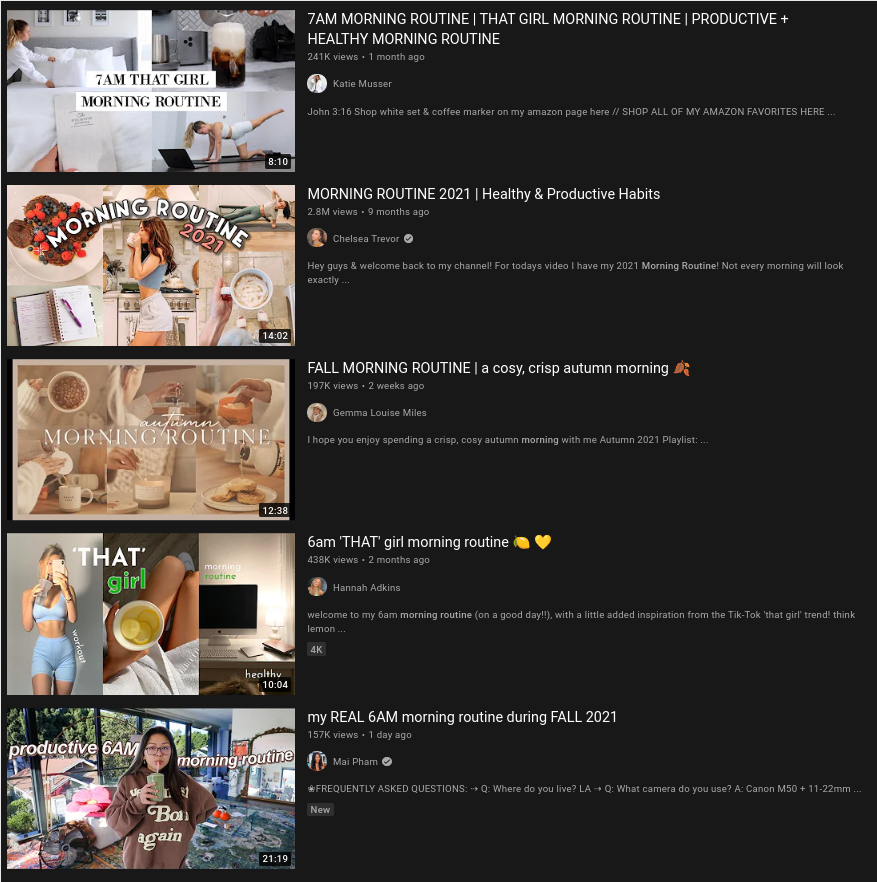
\includegraphics{mr1}
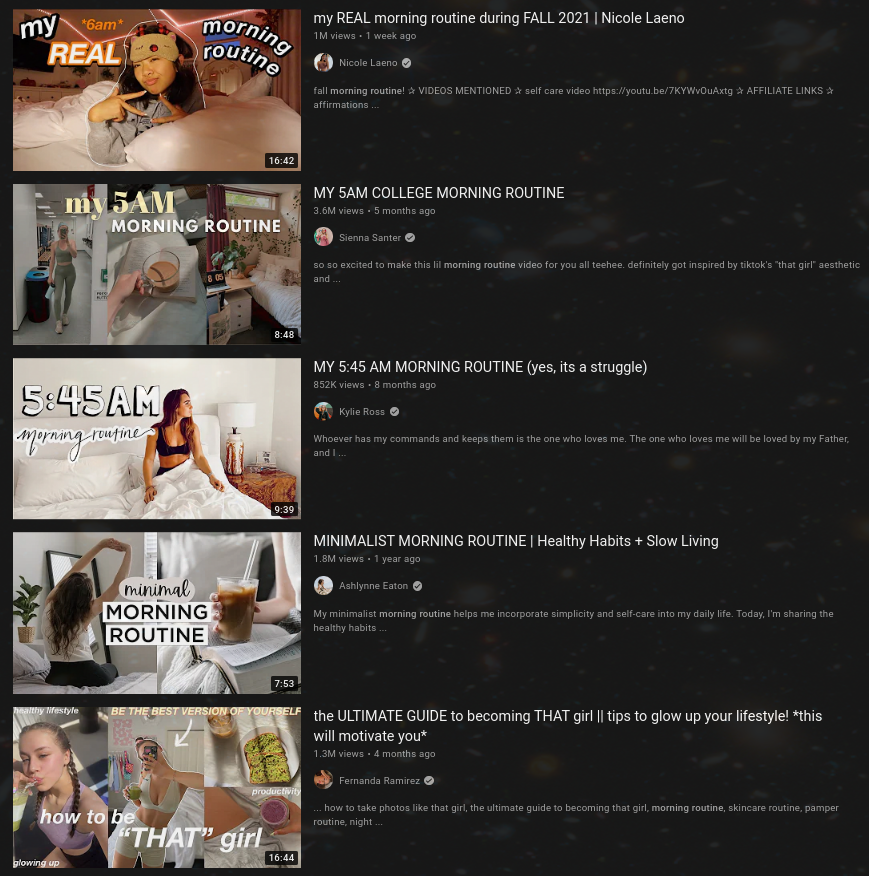
\includegraphics{mr2}

There's an endless supply of these videos that seem to follow the same general structure. The title will be something like: \\
\\
\textit{My 05:00AM Healthy <current year> Productive Morning Routine for Healthy Living and Productivity! *inspirational* *motivational*} 
\\\\
The thumbnail will contain a lot of beige and light colors that looks like it's from some interior design catalog.
\\\\
The contents of the video will be a subset of

\begin{itemize}
    \item
        Waking up really early
    \item
        Beige colors
    \item
        Yoga
    \item
        Cold Brew/Matcha Tea/Green smoothie in a jar
    \item
        Bullet-journaling
    \item
        Gratitude-journaling
    \item
        Meditation
    \item
        Plants
    \item
        Skincare
    \item
        Reading Self-help books
    \item
        Ass Workout
    \item
        Vegan
    \item
        Pretty cereal bowls with fruit and nuts
    \item
        Highlighting with markers
    \item
        Avocado
    \item
        MacBooks
    \item
        Inspirational quotes
    
        
\end{itemize}

And of course, all the videos are made by women.
\\
\\
The aesthetic is nothing new. Beige colors, journals, things in jars, yoga pants, etc. is something you'll see on most of social media. Which indicates this is mostly a special case of something more general. Some of the videos mention a concept called "that girl", which upon being googled returns: 

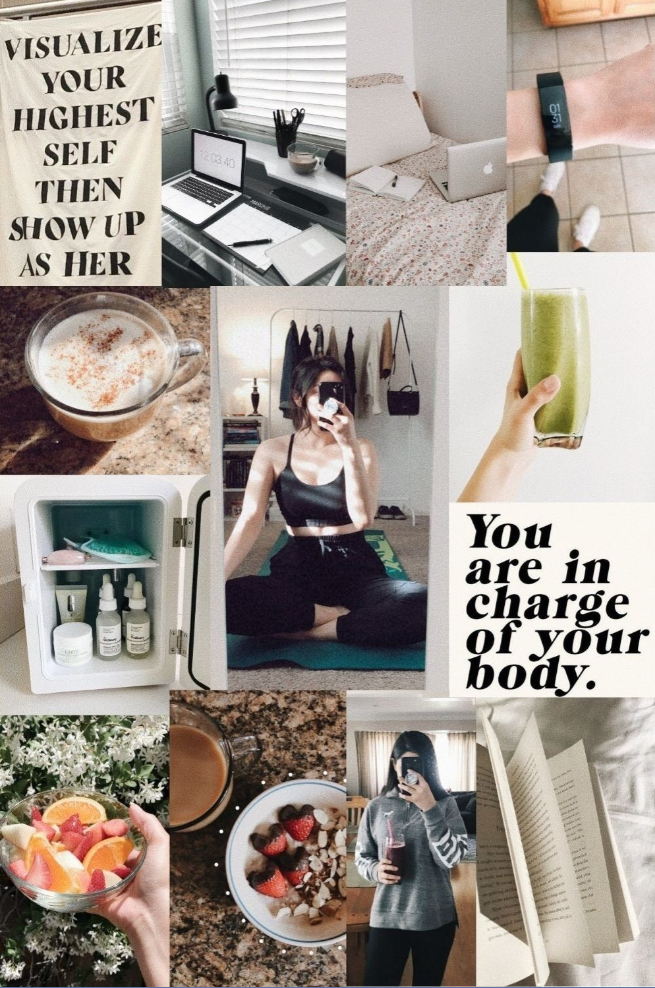
\includegraphics{tg1}

%Given the existence of this concept handle and the fact that a lot of the videos feel the need to specify "my *real* morning routine" or "my *realistic* morning routine" it seems that this trope is has already bubbled up into the collective consciousness of social media women.\\\\
It's a familiar argument that social media is about people flexing how great their lives are, and obviously this is sort of what's going on here. What interests me is how women-specific some of the behaviors are. Being healthy and productive is a big status object among men as well as among women, but I guess drinking green things from jars, doing yoga, and having a bullet journal are the status signals women use? 
\\\\


\end{document}
